\section{Glass RPC SDHCAL}
Contact person: Imad Laktineh (email: laktineh@IPNL.IN2P3.FR)
\subsection{Introduction}

Hadronic calorimeter (HCAL) plays an essential role in PFA-based experiments as
those proposed for the ILC. It allows to separate the deposits of charged and
neutral hadrons and to precisely measure the energy of the neutrals. The
contribution of the neutrals to the jet energy, around 10\% on average,
fluctuates in a wide range from event to event, and the accuracy of the
measurement is the dominant contribution to the particle flow resolution for jet
energies up to about \unit[100]{GeV}. For higher energies, the performance is
dominated by confusion, and both topological pattern recognition and energy
information are important for correct track cluster assignment.
High-granularity hadronic calorimeter is thus needed to achieve excellent jet
energy resolution.

HCAL proposed for both projects of ILC (ILD and SiD), are sampling calorimeters
with steel as absorber and scintillator tiles or gaseous devices with embedded
electronics for the active part. The steel was chosen due to its rigidity which
allows to build self-supporting structure without auxiliary supports (dead
regions). Moreover, the moderate ratio of hadronic interaction length
($\lambda_I = \unit[17]{cm}$) to electromagnetic radiation length ($X_0 = \unit[1.8]{cm}$) of
iron, allows a fine longitudinal sampling in terms of $X_0$ with a reasonable
number of layers in $\lambda_I$, thus keeping the detector volume and readout
channel count small. This fine sampling is beneficial both for the measurement
of the sizable electromagnetic energy part in hadronic showers as for the
topological resolution of shower substructure, needed for particle separation.

For the ILD project we propose gaseous detectors for the HCAL active layers: The
Resistive Plate Chamber (RPC). This is motivated by the excellent efficiency
and very good homogeneity the gaseous detectors could provide. Another
important advantage of gaseous detectors is the possibility to have very fine
lateral segmentation. Indeed, in contrast to scintillator tiles, the lateral
segmentation of gaseous devices is determined by the electronics readout used to
read them. Active layer thickness is also of importance for what concerns the
ILC hadronic calorimeter to be placed inside the magnetic field. Highly
efficient gaseous detectors can indeed be built with a thickness of less than
\unit[3]{mm}.

To obtain excellent resolution of hadronic shower energy measurement using a
binary readout, a lateral segmentation of few millimeters is needed. This
however leads to a huge number of electronics hardly affordable for the future
ILC hadronic calorimeters. $\unit[1\times 1]{cm^2}$ cells were found to be a good compromise
that still provides very good resolution at moderate energies. However,
simulation studies show that saturation effects are expected to show up at
higher energies ($> \unit[50]{GeV}$). This happens when many particles cross
one cell in the center of the hadronic shower. To reduce these effects, the
choice of multi-threshold electronics (Semi-Digital) readout was envisaged to
improve on the energy resolution by exploiting the particle density in more
appropriate way.

High-granularity calorimeters imply however a huge number of electronics
channels to operate them. This has two important consequences. The first is the
power consumption and the resulting increase of temperature which affects the
behavior of the active layers. The other consequence is the number of service
cables needed to power, read out these channels. These two aspects can
deteriorate the performance of the HCAL and destroy the principle of PFA if
they are not addressed properly.

The R\&D pursued by the SDHCAL-GRPC groups has succeeded to pass almost all the
technical hurdles of the PFA-based HCAL. The SDHCAL-GRPC groups have succeeded
to build the first technological prototype of these new-generation calorimeters
with 48 active layers of GRPC, $\unit[1]{m^2}$ each. The prototype validates the concept
of high-granularity gaseous detector and permits to study the energy resolution
of hadrons one can obtains with such calorimeter.


\subsection{Readout Electronics}

The readout electronics of the two Semi-Digital HCAL (SDHCAL) projects were
developed in common. An ASIC called HARDROC was first developed to read out the
GRPC detectors proposed for the ILD project. To solve the problem of
connections related to the high number of electronics channels, the option of a
detector embedded electronics using the DAISY chain scheme was chosen and
Printed Circuit Board (PCB) were conceived for the readout of large detectors
GRPC.

\subsubsection{Front-end ASIC}

The HARDROC chip (HR) implements a multi-threshold readout which integrates the
functionalities of amplification, shaping, digitization, internal triggering and
local storage of the data. Each of its 64 channels consists of a fast low
impedance current preamplifier with 8-bit variable gain (in the $[0,2]$ range)
followed by 3 fast shapers (\unit[15]{ns} shaping time). A low offset discriminator is
present on each path and the three corresponding thresholds establish the
multi-level readout. The thresholds are set using three integrated 10-bit
Digital to Analog Converters (DAC). The outputs of the three discriminators are
then encoded 3-to-2 bit and stored in an internal digital memory latched by a
trigger event.

A trigger is generated when one of the lowest level discriminators is fired but
can also be configured on the other thresholds. A frame consists of the 64
encoded discriminator outputs, plus a 24-bit time-stamp and a chip identifier is
stored after a trigger is received. Noisy channels could be easily masked via
the configuration parameters control. In order to avoid fake triggers produced
by noisy channels, the output of each discriminator can be switched off from the
trigger generator logic via the configuration parameters control (Slow Control
hereafter) commands. The response of all the channels can be calibrated by
injecting an analog signal through an integrated $\unit[2\pm 0.02]{pF}$ input test
capacitor; this is a useful tool to make the response of the different channels
as uniform as possible~\cite{1748-0221-6-02-P02001}.

The ASIC contains a 127-frame long digital memory. This allows to work in a
triggerless mode and keep all the data accumulated during the bench crossing.
Once the memory is full the acquisition is stopped, the readout is performed
and the ASIC can start acquisition again. The Gray-coded time-stamp is derived
from an external \unit[5]{MHz} clock.

An essential feature of the HR is the possibility to be operated in the
power-pulsing mode (PP) that consists of switching off almost all
power-consumption functionalities in between the bench crossings (BC) of the ILC
electron beams. With the ILC duty cycle of one \unit[1]{ms} of BC every \unit[200]{ms}, this
mode allows a reduction factor of more than 100 of power consumption. Thanks to
this reduction, the temperature increase of the HCAL is moderate and only
simple cooling system is needed to operate it efficiently.

\subsubsection{Active Sensor Units}

To read out the $\unit[1]{m^2}$ detector of the SDHCAL, an electronic board with the
same size is needed. This electronic board is an important piece in the present
design. It hosts both the pick-up pads and the ASICs in addition to the
connections linking the pads to the ASICs and those among the different ASICs.
To ensure good transmission qualities and low cross-talk, 8-layer Printed
Circuit Board (PCB) is designed. Feasibility constraints, make the tasks of
circuit production, components soldering, testing and handling of the
assemblies, exceedingly difficult in the case of a single board of one square
meter. The solution of dividing that circuit into 6 smaller but more
manageable PCB was adopted. Each of these small ASUs hosts 24 chips to read out
$48\times 32$ pads of $\unit[1]{cm^2}$ each. This dressed PCB is dubbed Active Sensor
Unit (ASU). The base pattern connecting 64 pads arranged in a $8\times 8$ matrix
to the ASIC's pins is shown in Figure~\ref{fig:Calorimeter:SDHCAL_GRPC:asicPins}. This is identical to the
one used in the ASUs of the small GRPC chambers described in reference
\cite{1748-0221-6-02-P02001}. The routing of each input signal from its own pad up to chip pin
has been carefully optimized to reduce the cross-talk. All input signals are
laid out in the same analog signal layer witch is sandwiched between two GND
layers. The routing of digital signals was kept well separated from the vias
connecting signals from one layer to another. In the case of the GRPC related
ASU, the HARDROC base pattern is replicated $4\times 6$ times in the $\unit[33.33]{cm}
\times \unit[50]{cm}$ board. 4 \unit[1.6]{mm} diameter holes are present on the four
angles of a PCB to be used for fixation purposes as will be explained later.
The rooting was conceived so two of the ASUs can be associated to form one slab
hosting 48 ASICS. Each slab is then connected to one Detector InterFace board
(DIF). The connection between the DIF and the slab as well as the connection
of the two ASUs is performed thanks to tiny connectors allowing the
different clocks, signals as well as the power to circulate between the two
ASUs. Three slabs are then assembled to form the required electronics board.
To ensure the same electric reference level for the six ASUs, the GND layer of
the six ASUs is connected thanks to a copper gasket on all the common sides.
Similar schemes could be proposed for GRPC detectors with larger size.


\begin{figure}
\centering
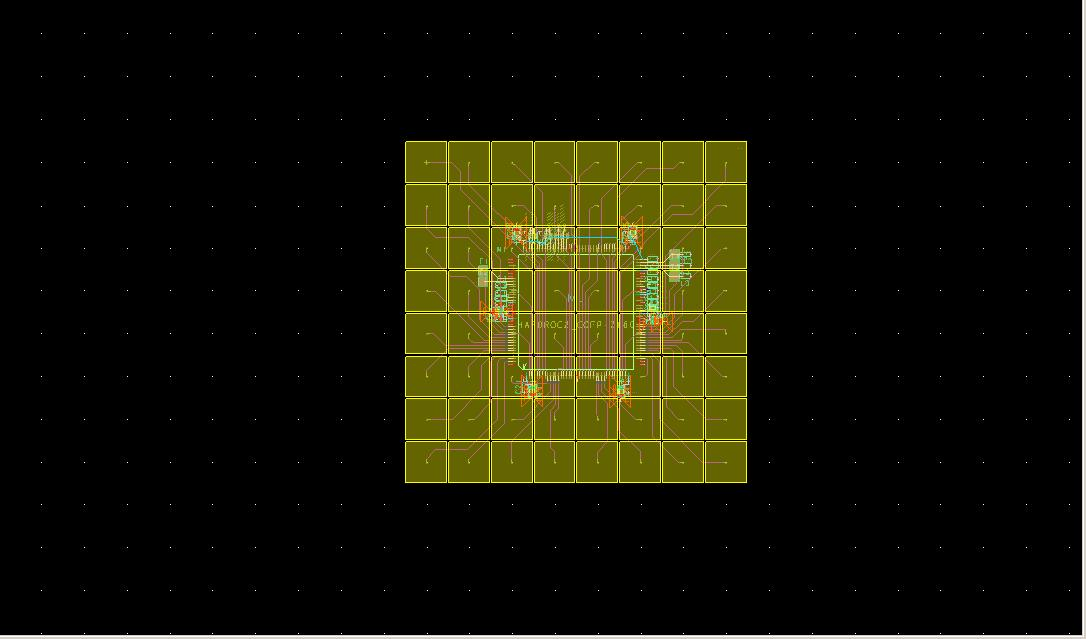
\includegraphics[width=.7\columnwidth]{Calorimeter/SDHCAL_GRPC/figures/HR2_base.jpg}
\caption{Pads connection to the ASIC's pins}
\label{fig:Calorimeter:SDHCAL_GRPC:asicPins}
\end{figure}


\subsubsection{Front-end and back-end boards}

The interface between the ASUs and the data acquisition system (DAQ) is realised
by the detector interface board called DIF. The main elements of the DIF is an
FPGA and USB, HDMI and SAMTEC connectors. It manages the control signals
(e.g. clock, busy/ready, external/internal trigger, power-pulsing) and
supply power to the ASICs and also performs the readout of the ASIC memories.
DIFs are read out by other FPGA-based boards called Data Concentrator Cards
(DCC). They can be connected up to 9 DIFs through HDMI links and are controlled
by a synchronous DCC (or SDCC). The SDCC can connects to up to 9 DCCs to which
it distributes the clock and the commands. It is also connected to the computer
network for the user to control the DAQ.

In the case of Micromegas ASUs, a small additional board called inter-DIF is
used between the DIF and ASU to provide the high voltage to the meshes and drift
electrode.


\subsubsection{Acquisition Software}

To exploit the data collected by the SDHCAL detectors an acquisition software
was developed. This software is organized in three parts. The first one allows
to access the hardware devices (DIF, SDCC) through an FTDI chip associated to
each of these devices. It transmits the configurations parameters to ASICs
through these devices and collect the data as well. The second part is the
configuration data base. It gives the possibility to store and retrieve all
parameters needed by the DAQ system. The database itself is hosted on an Oracle
server at CC IN2P3 (Villeurbanne, France). To interface this SQL database with
the DAQ software and to allow users to insert and query data without knowledge
of SQL, a C++ library has been written. A special care was taken to allow to
download the parameters associated to a given parameters of the prototype
(roughly 550000 parameters) in few seconds. The third part concerns the data
collection. Data from different DIFs may be readout at a different times but
will have the same Bench Crossing IDentifier (BCID) for a given trigger. The
logical way to keep synchronicity is to store in a BCID indexed map the buffers
of all read DIFs but it requires to man-age memory allocation, access and
cleaning. This was achieved thanks to the abilities offered by recent Linux
kernels to use file based shared memory. In addition, whenever several
computers are involved in the data taking, as it is the case for the SDHCAL
prototype, a communication framework is needed. The CMS data acquisition XDAQ
framework was chosen. This provides communication tools with both binary and
XML, an XML description of the computer and software architecture, a web-server
implementation of all data acquisition application and a scalable event builder.
A monitoring system was also developed to have a online follow-up of the
acquisition during data collection.

\subsection{GRPC-SDHCAL for ILD}
\subsubsection{Detector Development}

The structure
of GRPC proposed as an active layer of the HCAL proposed for ILD is shown in
Figure~\ref{fig:Calorimeter:SDHCAL_GRPC:chamber}. It is made out of two glass plates of \unit[0.7]{mm} and \unit[1.1]{mm}
thickness. The thinner is used to form the anode while the the thicker forms
the cathode. Ceramic balls of \unit[1.2]{mm} diameter are used as spacers between the
glass plates. The balls are glued on only one of the glass plates. In
addition to those balls, 13 cylindrical fiber-glass buttons of \unit[4]{mm} diameter
are also used. Contrary to the ceramic balls the buttons are glued to both
plates ensuring thus a robust structure.

Special spacers (ceramic balls) were used to maintain uniform gas gap of \unit[1.2]{mm}.
Their number and distribution were optimized to reduce the noise and dead
zones ($0.1 \%$). The distance between the spacers (\unit[10]{cm}) was fixed so that
the deviation of the gap distance between the two plates under the glass weight
and the electric force does not exceed \unit[45]{microns}. The choice of these spacers
rather than fishing lines was intended to reduce the dead zones ($0.1 \%$). It
was also aimed at reducing the noise contribution observed along the fishing
lines in standard GRPC chambers. The gas volume is closed by a \unit[1.2]{mm} thicks
and \unit[3]{mm} wide glass-fiber frame glued on both glass plates. The glue used for
both the frame and the spacers was chosen for its chemical passivity and long
term performance.

The resistive coating on the glass plates which is used to apply the high
voltage and thus to create the electric field in the gas volume was found to
play important role in the pad multiplicity associated to a mip \cite{1748-0221-6-02-P02001}.
To find the best coating for GRPC chambers many products were tested. Finally, a
new product based on two components was chosen. By changing the two components
ration one can obtain the needed surface resistivity. Commercial products like
Licron\texttrademark and Statguard\texttrademark which are used for Electro-Static
Discharge (ESD) applications were tried and few $\unit[1]{m^2}$ chambers were built
using those products and intensively tested. Both products failed to satisfy our
application either for long term stability under the high voltage (Licronusing
those products ) or due to the impossibility to obtain the surface uniformity
needed for our application (Statguardusing those products ). Eventually, two
products were identified, both of which are based on colloids containing
graphite. Both can be applied using the silk screen print method, which ensures
very uniform surface quality. One of these products is a single component paint
with a dry surface resistivity of $\unit[1-10] M\Omega/\square$. The second product
comes as two components which must be mixed by the user. The surface resistivity
may be adjusted over a wide range by changing the mix ratio. Both products
require baking at around $170^\circ$ C to attain a stable surface resistivity.
One product based on colloids containing graphite was finally selected. The
product can be applied using the silk screen print method, which ensures very
uniform surface quality. In addition, the product is made of two components and
it was found that by changing the mix ratio the surface resistivity may be
adjusted over a wide range.

The measured surface resistivity at various points over a $\unit[1]{m^2}$ glass coated
with the previous paint showed a mean value of $\unit[1.2]{M\Omega/\square}$ and a
ratio of the maximum to minimum values of less than 2. A study was also made of
the repeatability of the surface resistivity between different mix batches. It
was found that surface resistivity in the range $\unit[0.5-2]{M\Omega/\square}$ could be
reliably reproduced. For $\unit[1]{m^2}$ GRPCs the painting is applied on the whole
glass plate except for \unit[3]{mm} from the edges. This distance, corresponding to the
frame width, was optimized so the dead zone of the detector is reduced while
external sparks due to the presence of the metallic cassette in the vicinity is
completely eliminated.

Another important aspect of this development concerns the gas circulation within
the GRPC taking into account that for ILD SDHCAL gas outlets should all be on
one side. A genuine system was proposed. It is based on channeling the gas
along one side of the chamber and releasing it into the main gas volume at
regular intervals. A similar system is used to collect the gas on the opposite
side. A finite element model has been established to check the gas
distribution~\cite{Bedjidian2010120}. The simulation confirms that the gas speed is
reasonably uniform over most of the chamber area.


In order to improve on the gas distribution in large chambers taking into
account the requirement that both gas outlets should be on the same side of the
detector to satisfy all possible mechanical structures proposed for ILD
hadronic calorimeter, new schemes were studied. The one we finally adopted
allows us to improve the gas distribution by channeling the gas along one side
of the chamber and releasing it into the main gas volume at regular intervals
thanks to \unit[1.2]{mm} diameter PEEK\texttrademark tubes fixed \unit[2]{cm} from the
chamber side. A similar system is used to collect the gas at the other side of
the chamber. A finite element model has been established to check the gas
distribution~\cite{Bedjidian2010120}. The simulation confirms that the gas speed is
reasonably uniform over most of the chamber area. as can be seen in
Figure~\ref{fig:Calorimeter:SDHCAL_GRPC:gas_distribution}.

The GRPC and its associated electronics are housed in a special cassette which
protects the chamber and ensures that the readout board is in intimate contact
with the anode glass. The cassette is a thin box consisting of \unit[2.5]{mm} thick
stainless steel plates separated by \unit[6]{mm} wide stainless steel spacers. Its
plates are also a part of the absorber.

The electronics board is assembled thanks to a polycarbonate spacer which is
also used to fill the gaps between the readout chips and to improve the overall
rigidity of the detector. The electronics board is fixed on the small plate of
the cassette. Thanks to tiny screws and the new set is fixed on the other plate
which hosts the detector and the spacers. The whole width of the cassette is \unit[11]{mm}
with only 6 of them corresponding to the sensitive medium including the GRPC
detector and the readout electronics.


\begin{figure}
\centering
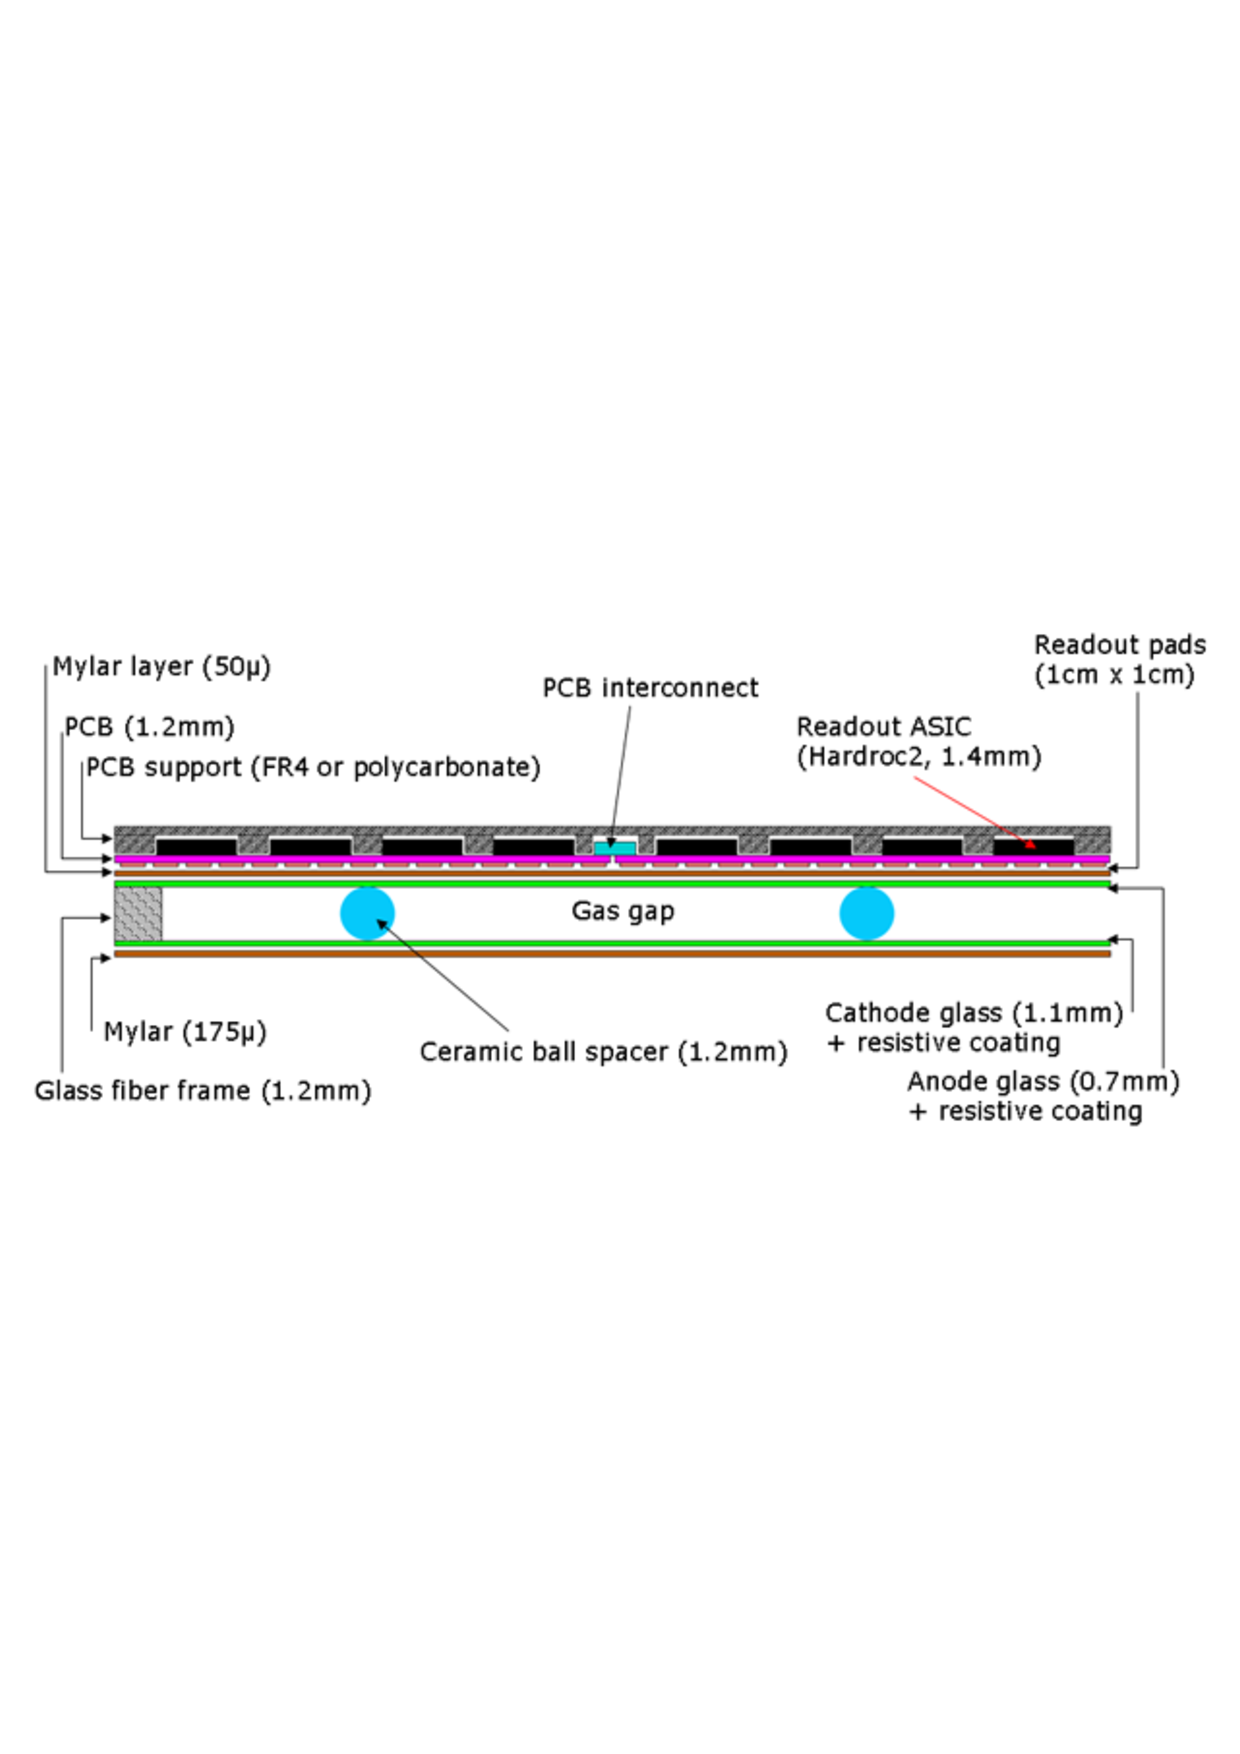
\includegraphics[width=0.70\textwidth]{Calorimeter/SDHCAL_GRPC/figures/chamber}
\caption{Cross-section through a $\unit[1]{m^2}$ chamber}
\label{fig:Calorimeter:SDHCAL_GRPC:chamber}
\end{figure}


\begin{figure}
\centering
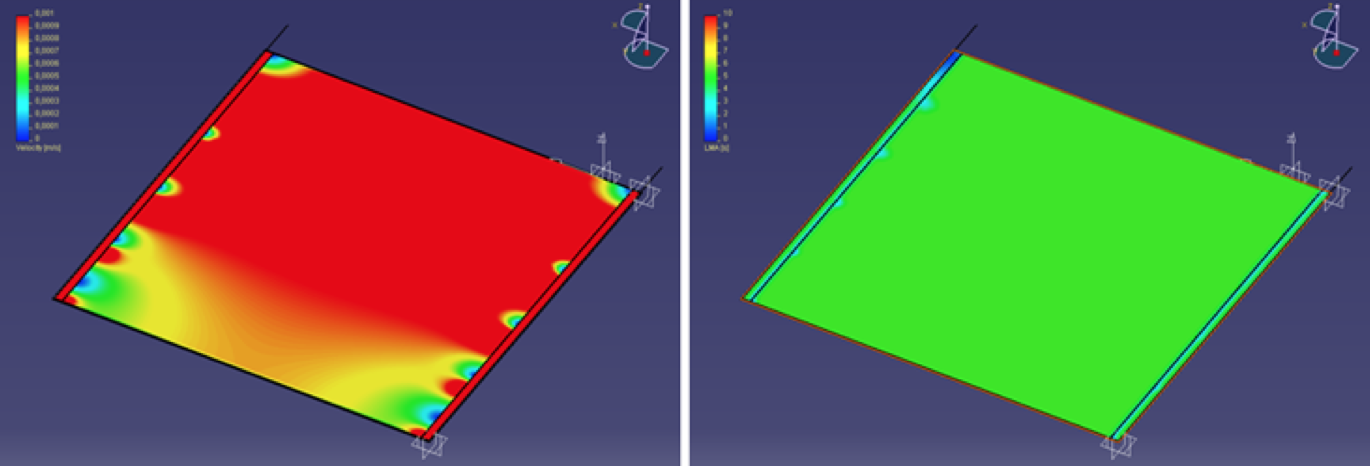
\includegraphics[width=.9\textwidth]{Calorimeter/SDHCAL_GRPC/figures/gas.png}
\caption{Left: Gas speed profile in the range \unit[0--1]{mm/s}; Right: Least mean age profile in the range \unit[0--10]{s}}
\label{fig:Calorimeter:SDHCAL_GRPC:gas_distribution}
\end{figure}

\subsection{Prototype}

A technological prototype corresponding to the SDHCAL option proposed in the ILC
LOI was built. 48 cassettes as the one described above were built. They
fulfilled a stringent quality control. It is worth mentioning that 10500 HR
ASICs were produced and tested using a dedicated robot for this purpose. The
yield was found to be higher than 92\%. The ASICs were then fixed on the PCBs
to make a $\unit[1]{m^2}$ and itself fixed on the cassette cover once successfully
tested.

The cassettes were inserted in a self-supporting mechanical structure that was
conceived and built in collaboration with the Spanish group of CIEMAT. The
structure is made of Stainless Steel plates of \unit[1.5]{cm} each. The plates were
machined to have an excellent flatness and well controlled thickness. The
flatness of the plates was measured using a laser-based interferometer system.
It was found that the flatness of the plates are less than 500 microns. This
results guarantees that for the SDHCAL V structure proposed for ILD, a tolerance
of less than \unit[1]{mm} is achievable.

The first cassettes were extensively tested using a cosmic-rays bench and later
particles beam at CERN. Both the efficiency and the multiplicity of the GRPC
cassettes were studied. These studies showed high efficiency and good
homogeneity and validated the cassette concept.

The prototype construction lasted less than 6 months. A commissioning test at
CERN in 2011 allowed to understand the whole system behavior. More precisely a
problem related to the acquisition system of the more than 430000 channels was
found and fixed.

In parallel a single cassette was tested in a magnetic field of 3 Tesla (H2 line
at CERN) applying the power-pulsed mode. The TB results indicated clearly that
the use of the power-pulsed mode in such a magnetic field is possible. The
behavior of the detector (efficiency, Figure~\ref{fig:Calorimeter:SDHCAL_GRPC:Eff}, multiplicity, Figure~\ref{fig:Calorimeter:SDHCAL_GRPC:Mult}) was found to be similar to
those obtained in the absence of both the magnetic field and the power-pulsed
mode.

In April 2012 the prototype was exposed to pion, muon, electron beams of both
the PS and the SPS of CERN (Figure~\ref{fig:Calorimeter:SDHCAL_GRPC:prototype}). Power-pulsed mode was applied to the
whole prototype using the beam cycle structure (\unit[0.3]{ms} time duration for the PS
beam and \unit[9]{s} for the SPS beam every \unit[45]{s}). A basic water-based cooling system was
used to keep under control the temperature increase particularly in in the case
of the SPS where the consumption reduction is only 5 (to compare with a factor
of more than 100 in the ILC case). An acquisition mode simliar to that of the ILC was operated.
The data were collected continuously in a triggerless mode. The DAQ stops when
the memory of one ASIC is full. Data are then transferred to a storage station
and then the acquisition starts again. Figures~\ref{fig:Calorimeter:SDHCAL_GRPC:PP1} and \ref{fig:Calorimeter:SDHCAL_GRPC:PP2} show the efficiency and
pad multiplicity of the prototype GRPC chambers measured using the muon beam.

The SDHCAL prototype results obtained with a minimum data treatment (no grain
correction) show clearly that excellent linearity and good resolution could be
achieved on large energy scale as can be shown in Figures~\ref{fig:Calorimeter:SDHCAL_GRPC:Linearity} and ~\ref{fig:Calorimeter:SDHCAL_GRPC:Resolution}. Useless to
mention that the high granularity of the SDHCAL allows one to study thoroughly
the hadronic showers topology and to improve on the energy resolution by, among
others, separating the electromagnetic and the hadronic contribution. The
separation between close-by showers will also get big benefit thanks to the high
granularity on the one hand and to to the very clean detector response ( $< \unit[1]{Hz/cm^2}$ )
on the other hand. These two points are being worked and recent results confirm this.

The quality of data obtained during three weeks of data taking validates
completely the SDHCAL concept as proposed in the LOI. This is especially
encouraging since no gain correction was applied to the electronics channels to
equalize their response. However a gain correction mode is elaborated and tested
during the TB. It will be applied in the future to assess the effect of such
correction on the energy resolution.


\subsection{ILD Preparation}

The expertise acquired with the construction and
the commissioning of the technological prototype and the obtained results were
used to implement a realistic simulation of the ILD HCAL. Physics channels such
as the $\mathrm{t} \bar{\mathrm{t}}\mathrm{H}$ were studied using the SDHCAL option and results were found
identical to those obtained with the scintillator tile option despite the fact
that the jet energy reconstruction code was optimized for the latter.

In addition, the French groups participated actively in the HCAL part of the
ILC TDR (ILD part) by proposing a genuine mechanical structure for the hadronic
calorimeter (called V-structure). The V structure was conceived to eliminate
the projective holes and cracks so none of the particles produced close to the
detector centre could escape detection. The V structure has additional
advantages. It eliminates in principle the space between the barrel and the
Endcaps avoiding the shower deformation which results not only because of
this space but also of the different cables and services needed in CMS-like
mechanical structures. In this structure the different services such as the
gas tubes, data collection and electric cables of both the barrel and the
Endcaps are taken out from the outer radius side.Detailed studies have shown
that the deformation of this structure is extremely low and its robustness was
verified experimentally with the SDHCAL technological prototype built with a
self-supporting structure respecting the spirit of the V one. Services and
Integration issues were also worked out. Besides, realistic costing was
performed , based on the prototype experience.

\begin{figure}
\centering
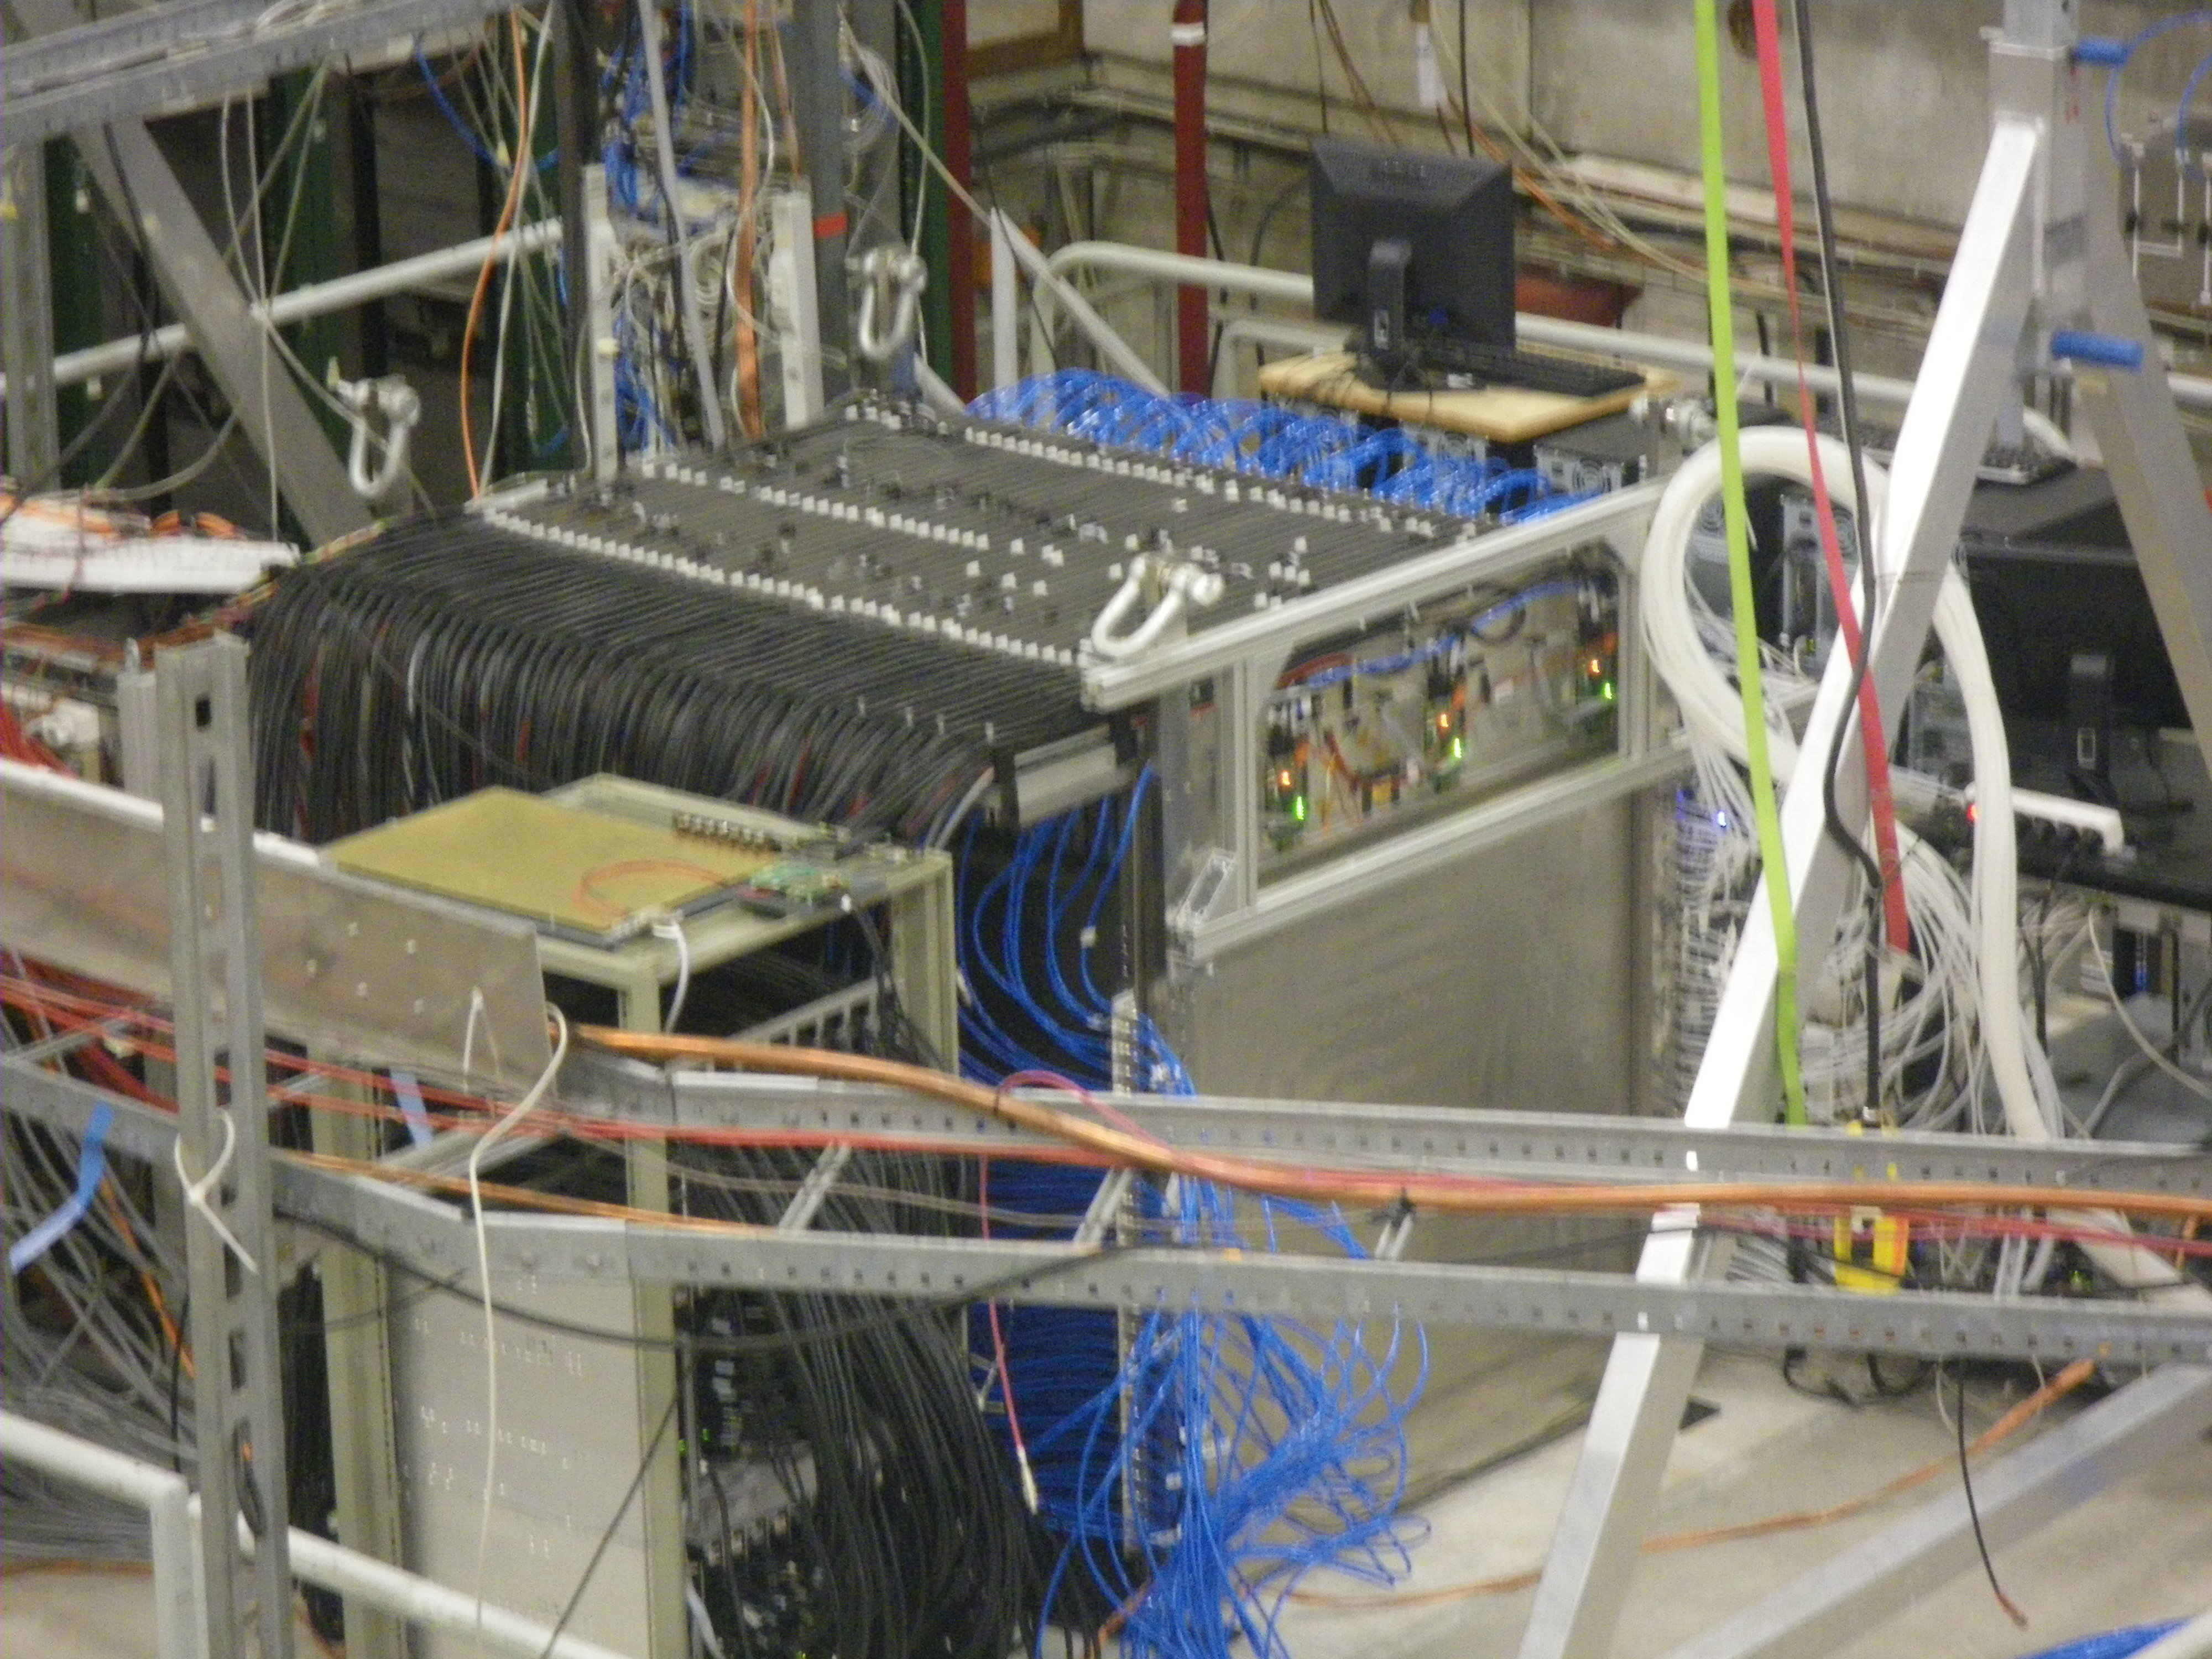
\includegraphics[width=0.50\columnwidth]{Calorimeter/SDHCAL_GRPC/figures/prototype.JPG}
\caption{Cross-section through a $\unit[1]{m^2}$ chamber.}
\label{fig:Calorimeter:SDHCAL_GRPC:prototype}
\end{figure}

\begin{figure}
\centering
 \begin{minipage}[t]{0.49\textwidth}
 \includegraphics*[width=\textwidth,keepaspectratio]{Calorimeter/SDHCAL_GRPC/figures/eff_layer_august_fit.pdf}
	\caption{Efficiency of the GRPC protoype}
 \label{fig:Calorimeter:SDHCAL_GRPC:Eff}
 \end{minipage}
\hfill
 \begin{minipage}[t]{0.49\textwidth}
 \includegraphics*[width=\textwidth,keepaspectratio]{Calorimeter/SDHCAL_GRPC/figures/mul_layer_august_fit.pdf}
 \caption{Pad multiplicity of the GRPC prototype. }
 \label{fig:Calorimeter:SDHCAL_GRPC:Mult}
 \end{minipage}
 \end{figure}

\begin{figure}
    \centering
 \begin{minipage}[t]{0.45\textwidth}
 \includegraphics*[width=0.7\textwidth,keepaspectratio]{Calorimeter/SDHCAL_GRPC/figures/BeamLine.jpg}
	\caption{GRPC setup in the CERN SPS-H2 line magnetic field.}
 \label{fig:Calorimeter:SDHCAL_GRPC:PP1}
 \end{minipage}
 \hfill
 \begin{minipage}[t]{0.45\textwidth}
 \includegraphics*[width=\textwidth,keepaspectratio]{Calorimeter/SDHCAL_GRPC/figures/BField_Efficiency_PowerPulsed.pdf}
 \caption{Efficiency scan over high voltage, with and without power pulsing. }
 \label{fig:Calorimeter:SDHCAL_GRPC:PP2}
 \end{minipage}
 \end{figure}

\begin{figure}
    \centering
 \begin{minipage}[t]{0.49\textwidth}
 \includegraphics*[width=0.7\textwidth,keepaspectratio]{Calorimeter/SDHCAL_GRPC/figures/Energy-Linearity-BEST.pdf}
	\caption{(a): Mean reconstructed energy for pion showers and (b): relative deviation of the pion mean reconstructed energy with respect to the beam energy.}
 \label{fig:Calorimeter:SDHCAL_GRPC:Linearity}
 \end{minipage}
\hfill
 \begin{minipage}[t]{0.49\textwidth}
 \includegraphics*[width=\textwidth,keepaspectratio]{Calorimeter/SDHCAL_GRPC/figures/Energy-Resolution-BEST.pdf}
 \caption{ $\frac{\sigma_{reco}}{E_{reco}}$ of the reconstructed pion energy $E_{reco}$ as a function of the beam energy. }
 \label{fig:Calorimeter:SDHCAL_GRPC:Resolution}
 \end{minipage}
 \end{figure}


\subsection{Recent Milestones}

\subsection{Engineering Challenges}
\subsection{Detector R\&D plans for the coming years}

Large GRPC of 1m$^2$ were developed and built for the technological prototype.
However, larger GRPC are needed in the future DHCAL with the largest one being
$\unit[290\times 91]{cm^2}$. These large chambers with gas inlet and outlet on one side need a
dedicated study to guarantee a uniform gas gap everywhere notwithstanding the
angle of the plate. It is necessary also to ensure an efficient gas distribution
as it was done for the $\unit[1]m^2$ chambers. To obtain this different gas distribution
systems were studied. A new scheme with two gas inlets and one outlet was found
to ensure an excellent homogeneity of the gas distribution. This system will be
used in the near future to build large detectors exceeding $\unit[2]{m^2}$. The readout
of such chambers needs also to be as efficient as the one of the technological
prototype $\unit[1]{m^2}$. An upgrade of the HR ASIC allowing larger dynamic range was
conceived, produced and successfully tested ~\ref{fig:Calorimeter:SDHCAL_GRPC:FSB}. The new ASIC (HR3)
allows to be directly addressed and easily bypassed in case of failure thanks to
the I2C protocol. In addition and contrary to the HR2, the 64 channels of the
new ASIC are independent which allows a better calibration procedure. In
addition to the previous challenges we need to improve on the interface boards
(DIF) needed to control the ASICs synchronization and data transfer. Indeed, the
space left between the active layer of one module and the cryostat is only \unit[5]{cm}.
This means that the DIF components should be optimized to cope with the volume
availability. A new design with new functionalities of the DIF is proposed. A
TPC/IP protocol is adopted for data transfer and a TTC one for the clock
synchronisation. A microprocessor implemented on the new DIF is in charge of
the communication between the ASICS and the DIF's FPGA. The new DIF is capable
to address up to 432 ASIC. New PCB design that allows to assemble few boards to
cover up to $\unit[3]{m^2}$ GRPC detector is being conceived. Care is taken to ensure
robust and flexible but still tiny connection between the different PCB to build
large one. Finally a new technique based on electron beam welding is being
tested to build a mechanical structure. This intends to reduce the steel
quantity used to assemble the absorber plates while guaranteeing a minimum
deformation. First attempts have taken place at CERN recently ~\ref{fig:Calorimeter:SDHCAL_GRPC:EBW} and
more study is ongoing to determine the best protocol one should follow to obtain
optimal results.

\begin{figure}
\centering
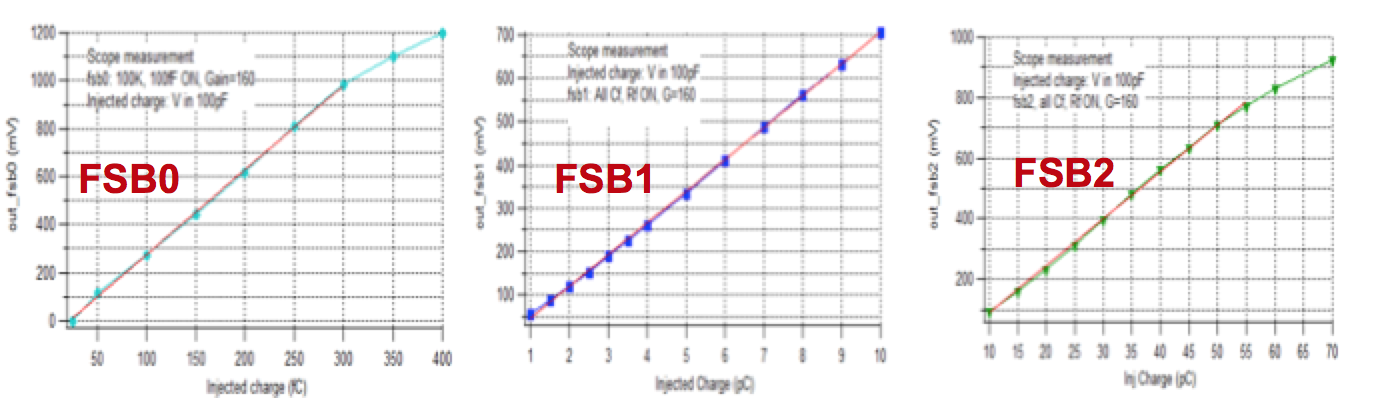
\includegraphics[width=0.90\textwidth]{Calorimeter/SDHCAL_GRPC/figures/FSB.png}
\caption{Dynmic range of the fast shapers associated to the three threshld of the new version of HARDROC.}\label{fig:Calorimeter:SDHCAL_GRPC:FSB}
\end{figure}

\begin{figure}
\centering
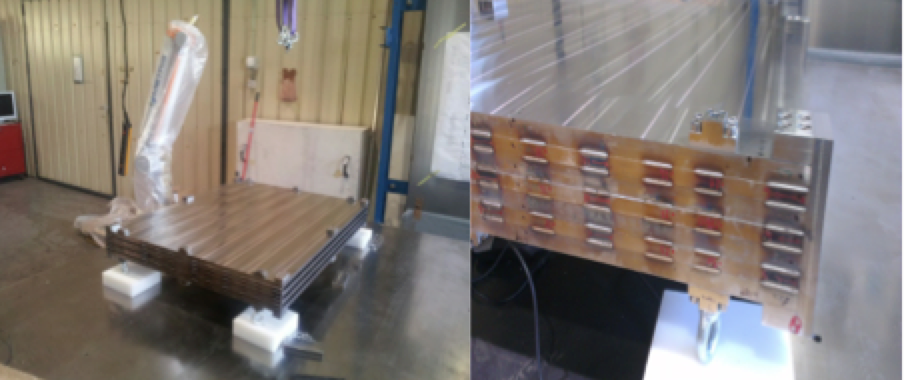
\includegraphics[width=0.90\textwidth]{Calorimeter/SDHCAL_GRPC/figures/EBW.png}
\caption{A prototype of an SDHCAL mechanical structure assembled using the electron beam welding technique.}\label{fig:Calorimeter:SDHCAL_GRPC:EBW}
\end{figure}
